\documentclass[11pt]{article}
\usepackage[a4paper, total={6.6in, 9.8in}]{geometry}
\usepackage{graphicx}
\graphicspath{ {./images/output/} }
\usepackage{caption}
\usepackage[english]{babel}
\usepackage{titling}
\usepackage{float}
% \usepackage{amsmath}
% \usepackage{minted}
% \usepackage{multicol}
% \usepackage{array}
% \usepackage{setspace}
% \usepackage{placeins}

% \usepackage{lipsum}

\title{Experiment 2 \\
    \textbf{Analysis of an Electroencephalogram (EEG) Signal}}
\author{}
\date{}

\pagenumbering{gobble}
\begin{document}
\vspace*{\fill}
\begin{center}

    \emph{Heaven's Light is Our Guide} \\
    \textbf{Rajshahi University of Engineering and Technology} \\

    \begin{figure}[H]
        \centering
        
\includegraphics[scale=.34]{images/RUET_logo.png}
        \label{fig:ruet_logo}
    \end{figure}
    \vspace{5mm}

    \textbf{Course Code}\\
    ECE 4144\\
    \vspace{3mm}
    \textbf{Course Title}\\
    Biomedical Engineering Sessional

    \vspace{5mm}
    \textbf{Experiment Date:} {August 06, 2025},\\
    \textbf{Submission Date:} {August 13, 2025}\\

    \vspace{5mm}
    \textbf{Lab Report 3: \\
        Experimental Observation of Various Features of an ECG
        Signal Collected from PhysioNet Public Dataset}

    \vspace{15mm}

    \begin{tabular}{c|c}
        \textbf{Submitted to} & \textbf{Submitted by} \\
        Md Mayenul Islam      & Md. Tajim An Noor     \\
        Assistant Professor   & Roll: 2010025         \\
        Dept of EEE, Ruet     &                       \\
    \end{tabular}

\end{center}
\vspace*{\fill}


\pagebreak
\maketitle

\vspace{-6em}

\section*{Objectives}
\begin{itemize}
    \item Analyze EEG signal characteristics and identify key waveforms.
    \item Understand standard electrode placement for EEG recording.
\end{itemize}

\section*{Theory}
Electroencephalography (EEG) records brain electrical activity using scalp electrodes. Signals originate from synchronized cortical neurons and are grouped into delta, theta, alpha, beta, and gamma bands, each reflecting different brain states. Amplitudes typically range from 10 to 100 microvolts. Proper electrode placement is essential for reliable data. EEG aids in assessing brain function and diagnosing conditions like epilepsy and sleep disorders~\cite{siuly2016eeg}.

\begin{figure}[H]
    \centering
    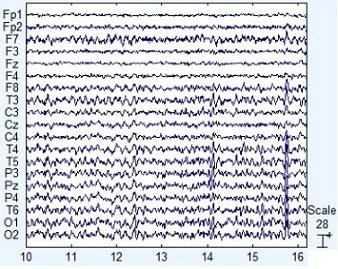
\includegraphics[width=.5\textwidth]{eeg.jpg}
    \caption{Sample EEG Signal\cite{eeg}}
\end{figure}

\subsection*{EEG Electrode Placement}
Basic EEG recording requires at least two electrodes: one active and one reference. For clinical assessments, 8 to 16 electrodes are typically used to ensure reliable data. The standard 10-20 system employs 21 electrodes placed at specific scalp locations. Advanced EEG setups may use up to 256 electrodes to achieve high spatial resolution.

\begin{figure}[H]
    \centering
    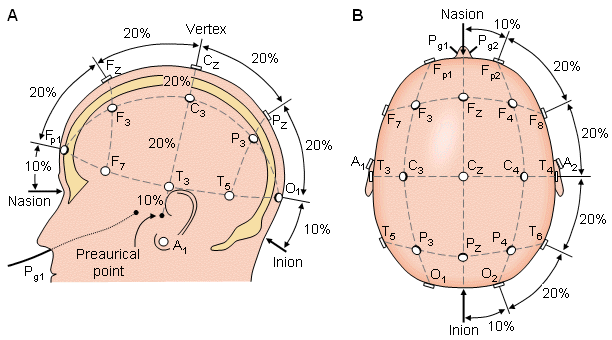
\includegraphics[width=.4\textwidth]{placement.png}
    \caption{EEG 10-20 Electrode Placement\cite{place}}
\end{figure}

\section*{EEG Signal Characteristic}
EEG signals vary by individual and brain state but are classified into frequency bands linked to specific activities:

\begin{table}[H]
    \centering
    \begin{tabular}{|c|c|l|}
        \hline
        \textbf{Band} & \textbf{Frequency (Hz)} & \textbf{Activity}            \\
        \hline
        Delta         & 0.5--4                  & Deep sleep                   \\
        Theta         & 4--8                    & Drowsiness, meditation       \\
        Alpha         & 8--13                   & Relaxed, awake (eyes closed) \\
        Beta          & 13--30                  & Alertness, concentration     \\
        Gamma         & 30--100                 & High-level cognition         \\
        \hline
    \end{tabular}
    \caption{EEG Frequency Bands and Activities\cite{siuly2016eeg}}
\end{table}

\subsection*{EEG Frequency Bands and Clinical Significance}
EEG frequency bands reflect brain states: delta/theta (sleep, drowsiness), alpha (relaxation), beta (alertness), gamma (cognition). Abnormal patterns—such as excess slow waves or altered alpha/beta rhythms—may indicate disorders like epilepsy, sleep issues, or brain injury~\cite{siuly2016eeg}.

\subsection*{EEG in Diagnosis}
EEG supports diagnosis of epilepsy, sleep disorders, encephalopathies, and brain death. It helps localize lesions, monitor anesthesia, and assess brain function~\cite{siuly2016eeg}.

\subsection*{EEG Signal Formation}
EEG signals originate from synchronized postsynaptic potentials in cortical neurons, mainly pyramidal cells. Quality depends on electrode placement, tissue conductivity, and noise reduction.

\section*{Discussion}
\addcontentsline{toc}{section}{Discussion}
EEG signals were analyzed theoretically due to lack of lab equipment. The focus was on signal origin, electrode placement, and frequency bands. Practical data collection was not performed.

\bibliographystyle{IEEEtran}
\renewcommand{\bibname}{References}
\addcontentsline{toc}{section}{References}
\bibliography{ref}

\end{document}
